\section{Análisis}

\subsection{Experimento 1}

\indent \indent Para este experimento planteamos un esquema cliente-servidor donde el cliente envía paquetes y el servidor solamente se encarga de reconocerlos.\\

\indent El objetivo era observar la evolución de la estimación del RTO desde el lado del cliente dependiendo del par de $\alpha$ y $\beta$ que se utilicen y en base a todas las combinaciones que se probaron, elegir las que a nuestro criterio nos dieran mejores resultados.\\

\indent Es fácil desprender de la definición del RTO que idealmente este valor debería coincidir con el RTT de la transmisión. Luego, esperábamos observar que a medida que se envían paquetes, el RTO estimado converge al valor del RTT.\\

\indent Como nos interesaba observar el impacto de estos valores en la progresión de la estimación del RTO, fijamos un valor de delay en 2 segundos cada vez que el servidor enviaba un ACK y no se definió probabilidad de dropeo. Así, nos asegurábamos un RTT de aproximadamente dos segundos (dado que ambos extremos de la conexión eran locales, el delay de la conexión podría despreciarse y el RTT dependería casi totalmente del delay forzado a mano a la hora del envío del ACK), de manera que se podía contrastar fácilmente en un gráfico, y además que todos los mensajes enviados eran correctamente reconocidos en tiempo y forma, sin dar lugar a retransmisiones.\\

\indent Con esto en mente, comenzamos a hacer corridas del experimento con diversas combinaciones de $\alpha$ y $\beta$. Consideramos suficiente hacer ochenta y un combinaciones, que surgen de elegir para ambas variables valores desde 0.1 a 0.9 aumentando en cada corrida en 0.1 la varible analizada y combinándola con los nueve valores de la otra variable.Si bien esto es arbitrario, probamos algunos pocos valores en los intevalos sin analizar y decidimos que aumentar la granularidad no nos daría cambios significativos en los resultados.\\

\indent Para analizar estos 81 resultados, partimos los datos en nueve gráficos\footnote{Aparte de estas imágenes, debajo de cada uno se encuentra un link a su versión interactiva, para poder apreciar mejor los datos.}, fijando cada valor de $\alpha$ y graficando las variaciones de los $\beta$.\\

\indent En todos los gráficos, aparte del resultado de cada $\beta$ con el $\alpha$ de dicha corrida, se encuentra una línea constante que representa el \textbf{RTT promedio} de cada corrida, que es el valor al que conjeturamos el RTO debería converger. Es notable que a pesar de haber fijado el delay en dos segundos, los RTT que se fueron obteniendo fueron ligeramente más pequeños, algo quizá atribuible a nuestra implementación. Sin embargo, dado que en todos los casos resultaba en valores casi constantes, consideramos que no enturbiaba la experimentación realizada.\\

\indent Dijimos que ibamos a seleccionar de estos valores aquellos que mejor nos parecían. El criterio utilizado para dicha selección consiste en un equilibrio entre dos cuestiones: en primer lugar, la velocidad de convergencia al RTT, suponiendo mejor una convergencia más rápida; y en segundo lugar, la estabilidad de la progresión una vez cerca del RTT, tratando de evitar aquellas con comportamiento errático. Debe entenderse entonces que se contemplan ambos aspectos en la elección (ligeramente subjetiva) de dichos valores de $\alpha$ y $\beta$, y que, por lo tanto, una corrida que por ejemplo converge antes, no es necesariamente la que seleccionamos.\\

\indent En los siguientes gráficos se puede observar la progresión de la estimación del RTO en función de la cantidad de paquetes enviados. En este experimento en particular la cantidad de envíos se condice con la cantidad de estimaciones del RTO, porque se forzó al cliente a que recién enviara otro paquete cuando hubiera recibido un mensaje de confirmación del servidor (cuyo envío en el servidor forzamos nosotros y que no es el ACK). Hicimos esto para tener más control en la corrida y en la obtención de los datos. Por esta razón, el eje x de las siguiente figuras podría entenderse tanto como paquetes enviados como cantidad de estimaciones del RTO.\\

\indent En cada gráfico, además, está fijado un $\alpha$ y se muestran las nueve curvas que surgen de combinar dicho $\alpha$ con los $\beta$. Diferenciada de las demás curvas en azul se puede percibir la curva que se corresponde con el par $\alpha$ $\beta$ elegido en cada gráfico.\\
\begin{center}
	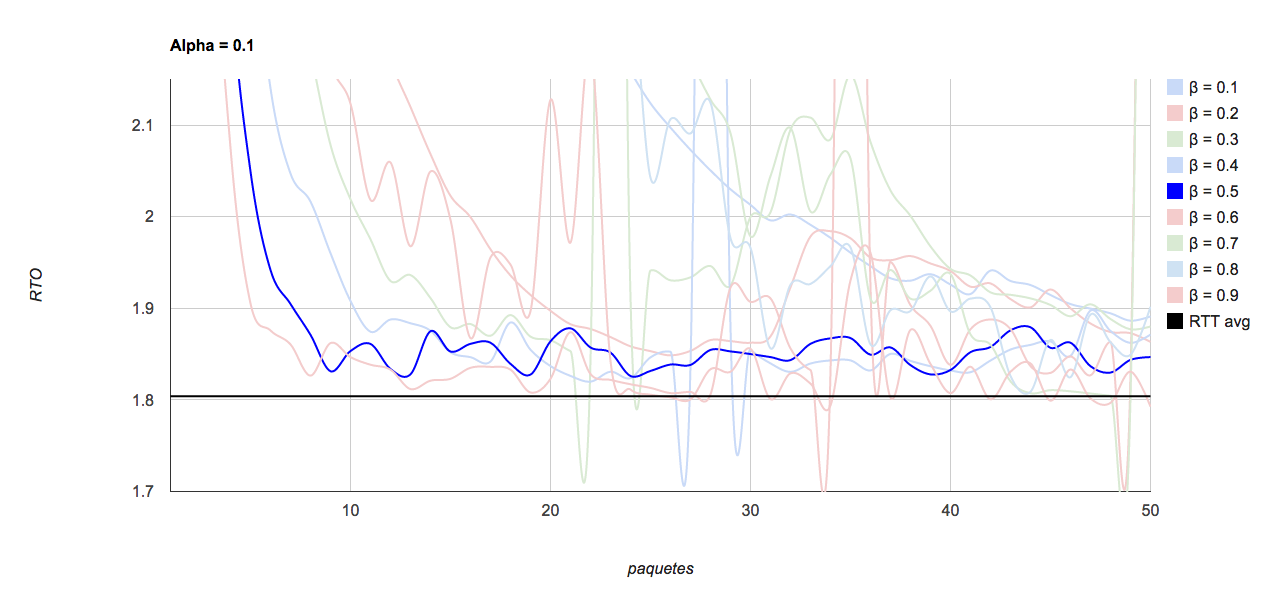
\includegraphics[scale=0.35]{graphics/rto_vs_paquetes_a_1.png}
	\textit{Gráfico interactivo en:} http://goo.gl/i3q8vd
\end{center}

\begin{center}
	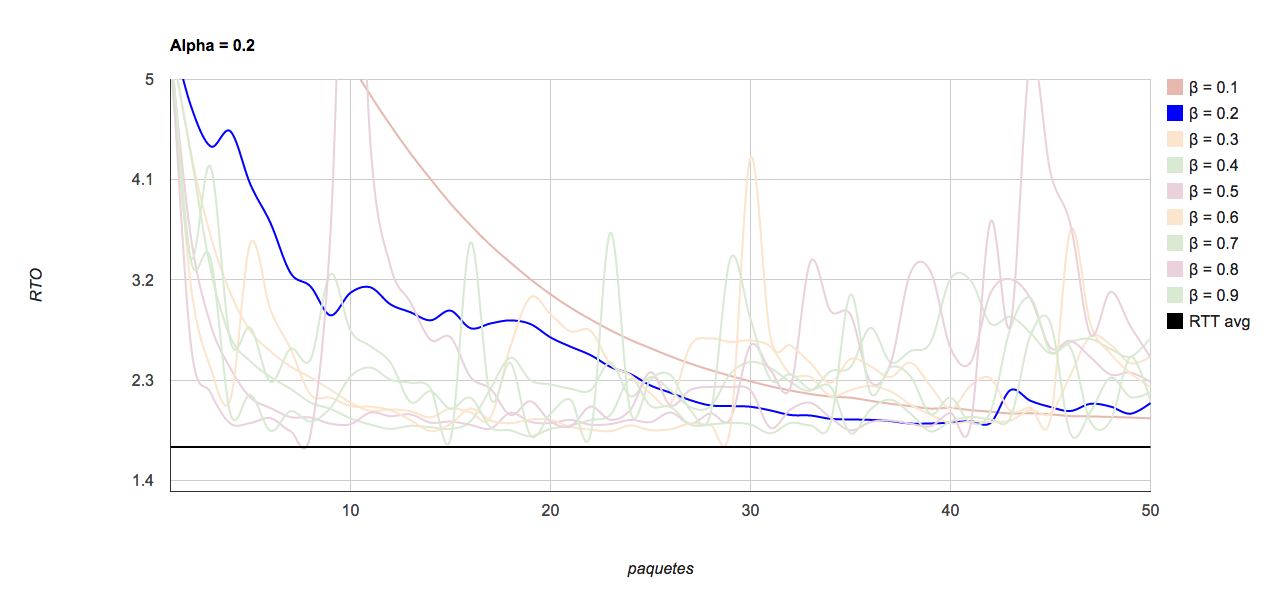
\includegraphics[scale=0.35]{graphics/rto_vs_paquetes_a_2.png}
	\textit{Gráfico interactivo en:} http://goo.gl/QS0NjO
\end{center}

\begin{center}
	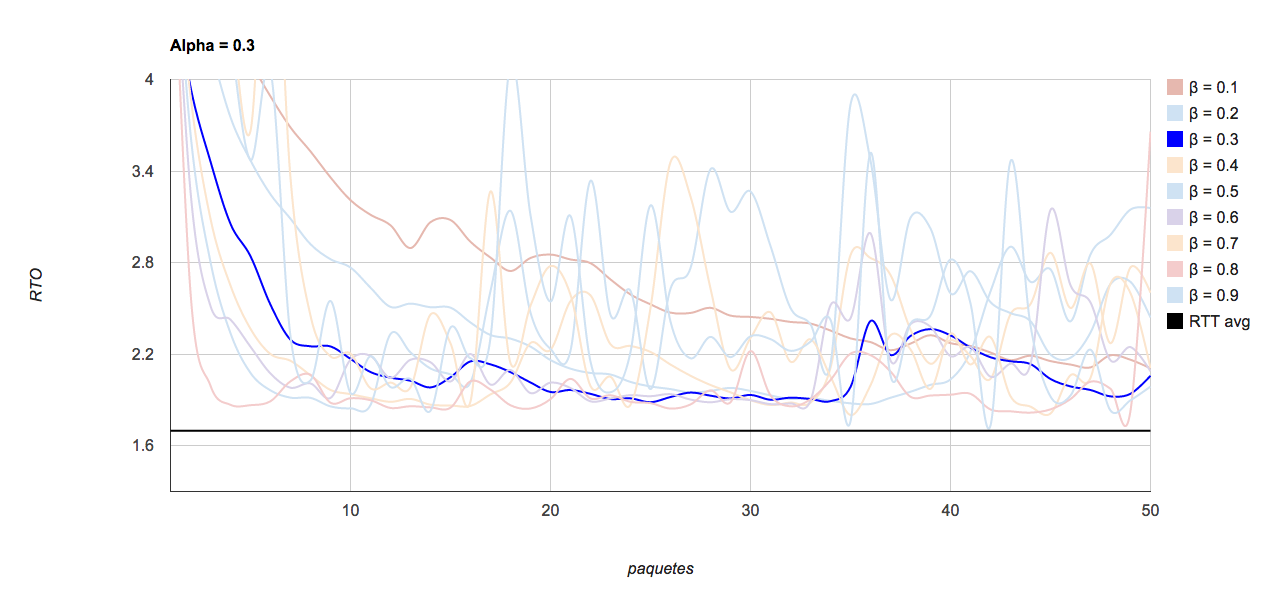
\includegraphics[scale=0.35]{graphics/rto_vs_paquetes_a_3.png}
	\textit{Gráfico interactivo en:} http://goo.gl/cmSyGd
\end{center}

\begin{center}
	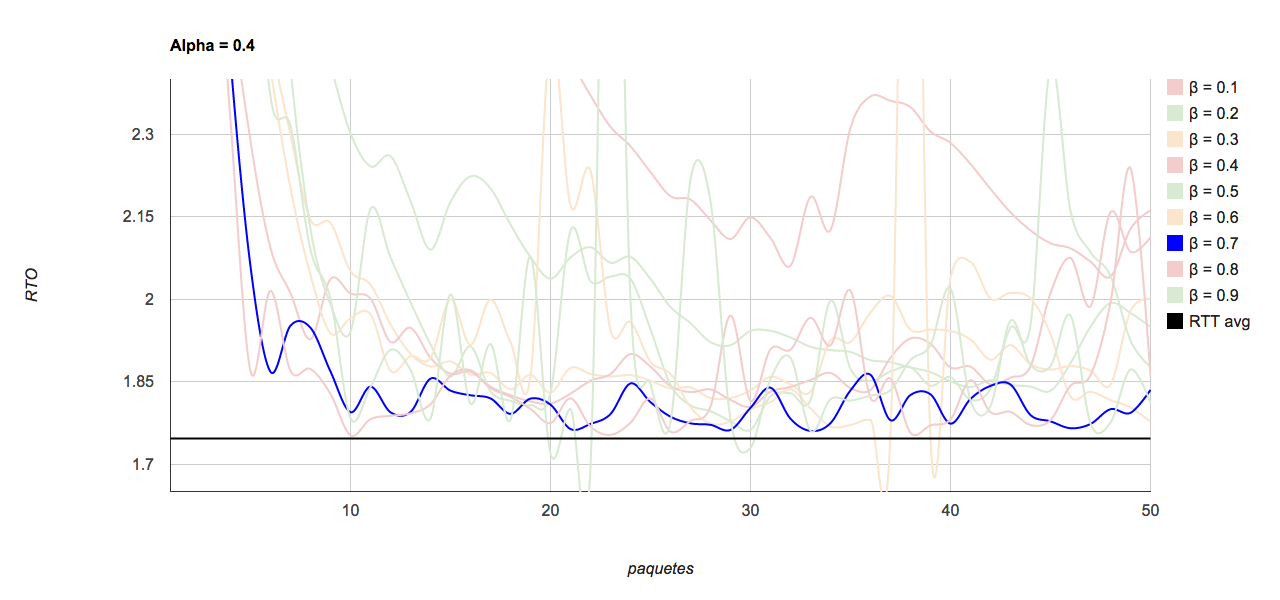
\includegraphics[scale=0.35]{graphics/rto_vs_paquetes_a_4.png}
	\textit{Gráfico interactivo en:} http://goo.gl/Db08yU
\end{center}


\indent Notar que estos primeros cuatro gráficos están a una escala más que pequeña que algunos de los que siguen a continuación. En particular, estos gŕaficos pueden resultar medio caóticos, pero dejan en claro que las curvas no son suaves sino que poseen varios picos. En esta escala pequeña queda un poco más claro el criterio de elección que hemos realizado, eligiendo en cada caso la curva y los $\alpha$ y $\beta$ que nos pareció que convergieron a un velocidad razonables y que además fueron los que más se estabilizaron cerca del RTT promedio.\\

\indent Es fácil también observar que todos decaen rápidamente de su valor inicial y se acercan al RTT y luego van fluctuando alrededor de dicho valor.\\

\indent Los siguientes dos gráficos tienen una escala un poco más grande. En ellos se puede ver claramente como la estimación del RTO va decreciendo hasta acercarse a un valor parecido al RTT para luego ir fluctuando cerca de ese valor:\\

\begin{center}
	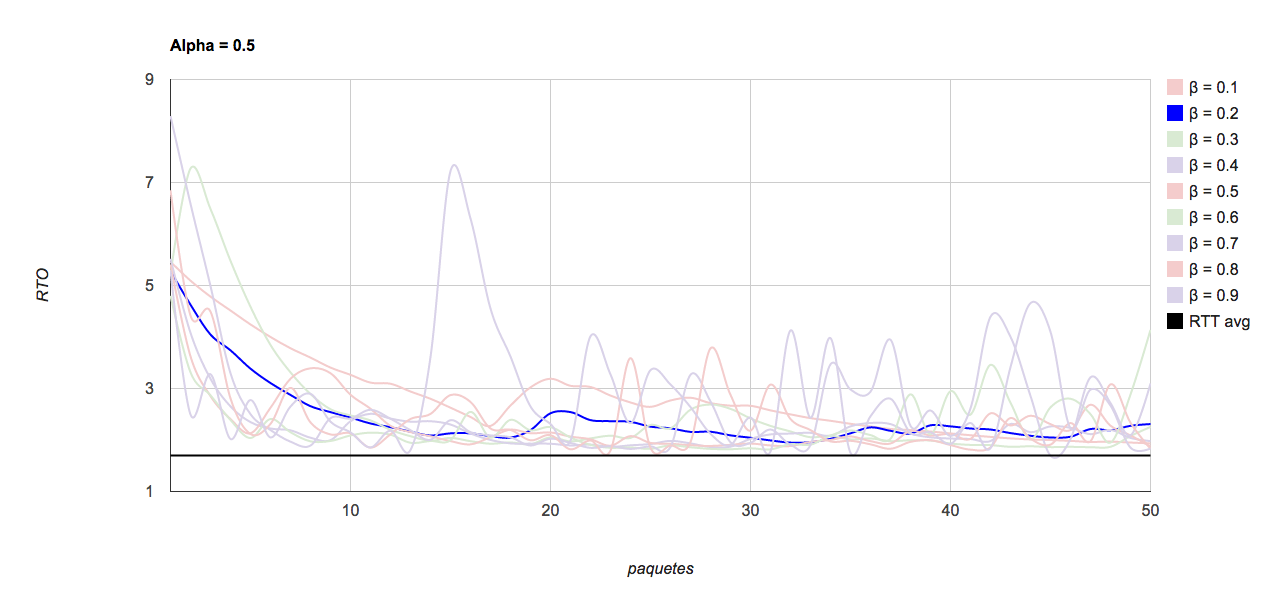
\includegraphics[scale=0.35]{graphics/rto_vs_paquetes_a_5.png}
	\textit{Gráfico interactivo en:} http://goo.gl/VNV8xF
\end{center}

\begin{center}
	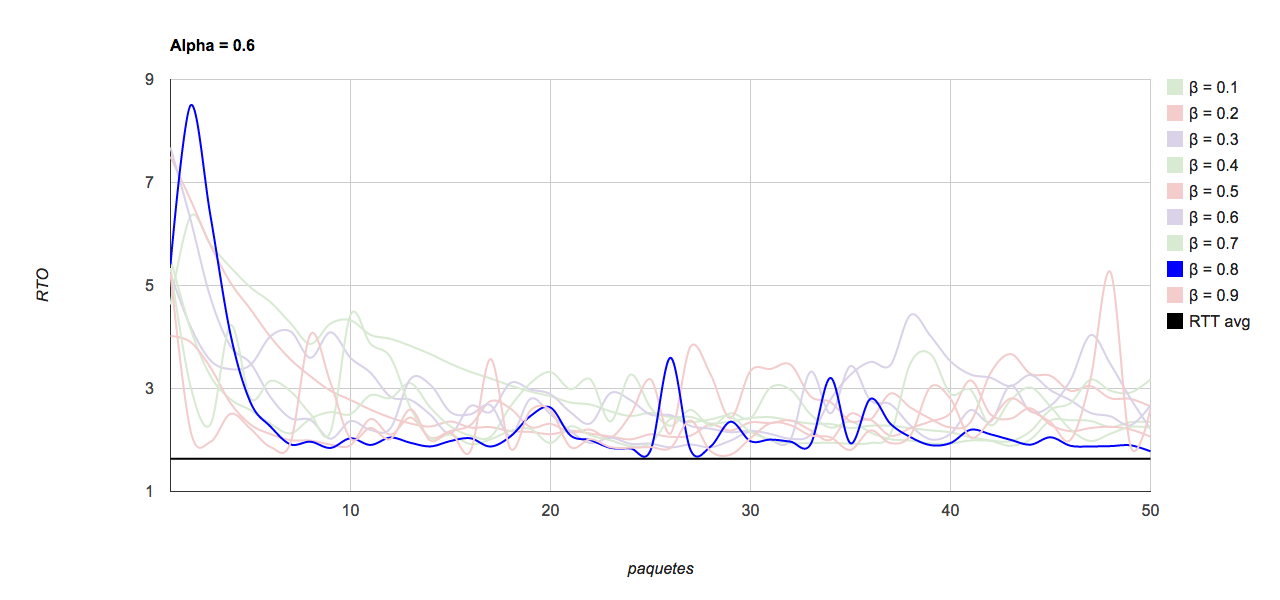
\includegraphics[scale=0.35]{graphics/rto_vs_paquetes_a_6.png}
	\textit{Gráfico interactivo en:} http://goo.gl/CN4joc
\end{center}


\begin{center}
	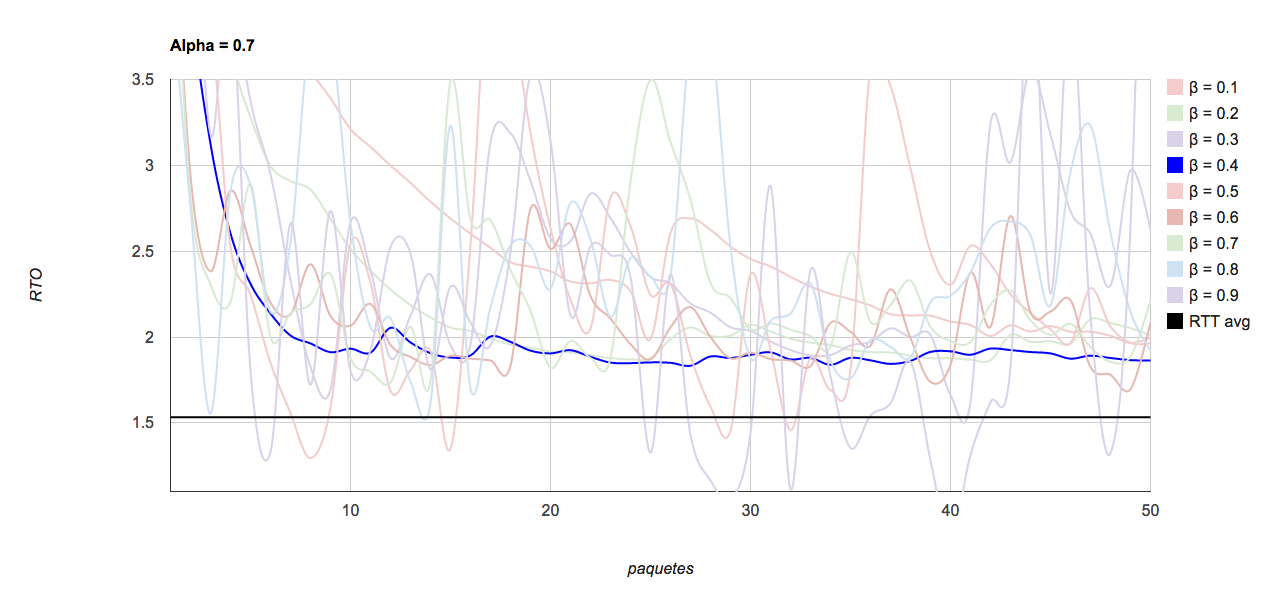
\includegraphics[scale=0.35]{graphics/rto_vs_paquetes_a_7.png}
	\textit{Gráfico interactivo en:} http://goo.gl/Gc93dU
\end{center}

\begin{center}
	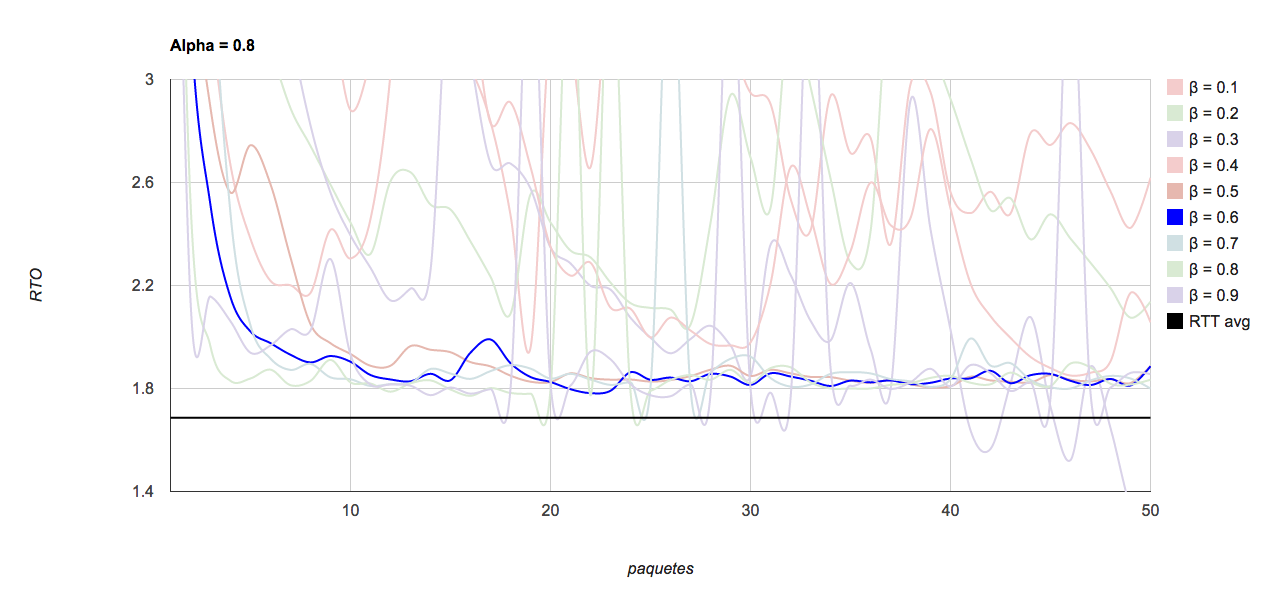
\includegraphics[scale=0.35]{graphics/rto_vs_paquetes_a_8.png}
	\textit{Gráfico interactivo en:} http://goo.gl/RGiQc0
\end{center}

\begin{center}
	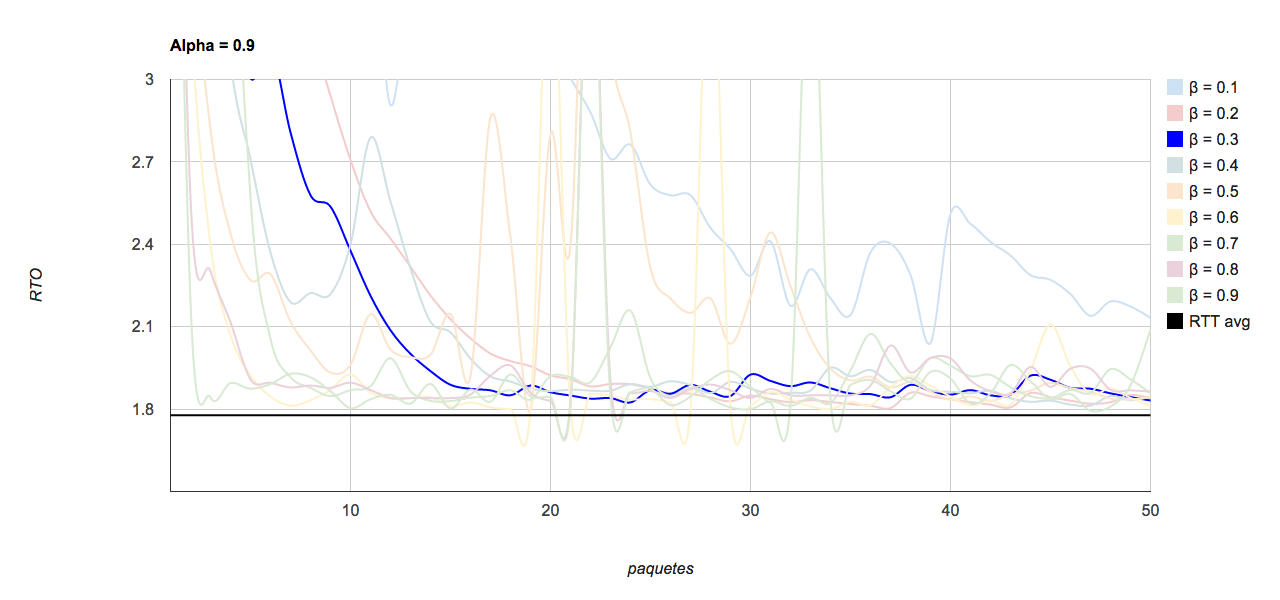
\includegraphics[scale=0.35]{graphics/rto_vs_paquetes_a_9.png}
	\textit{Gráfico interactivo en:} http://goo.gl/QXH7cA
\end{center}

\indent

\indent El siguiente gŕafico se corresponde con la contraposición de las curvas correspondientes a las $\alpha$ y $\beta$ elegidos de cada uno de los gŕafico.Comparando los resultados, concluimos que para nuestra experimentación los valores que mejores resultados nos dieron fueron $\alpha = 0.4$ y $\beta = 0.7$.\\ 

\begin{center}
	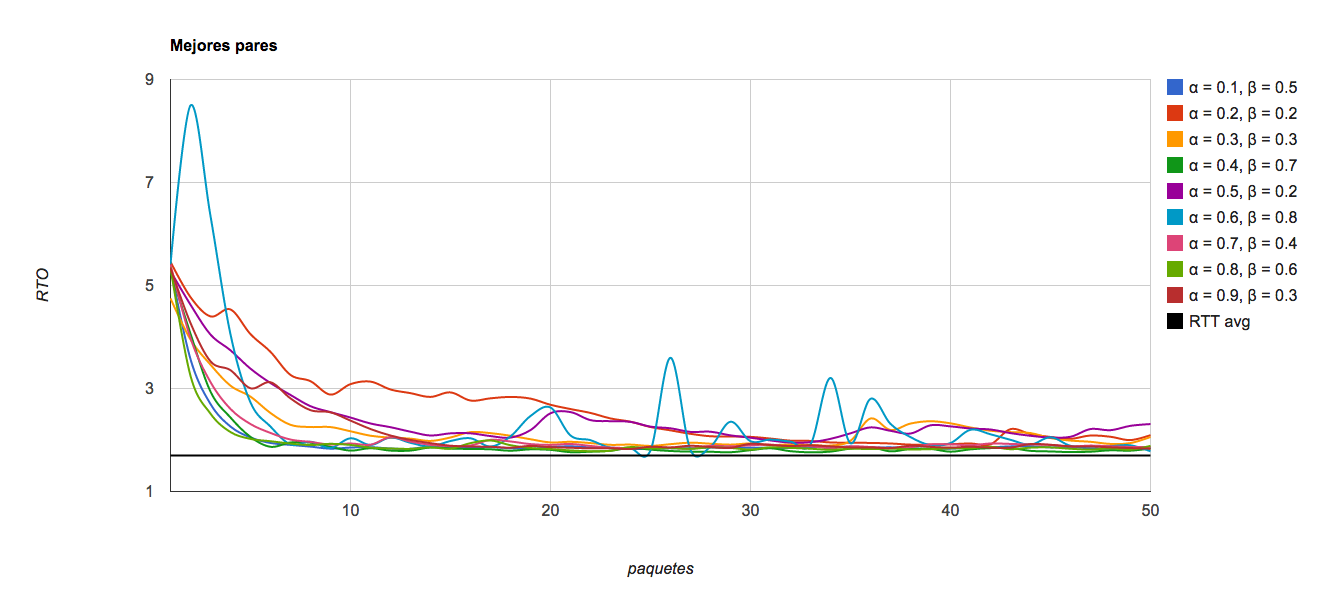
\includegraphics[scale=0.35]{graphics/best_pairs.png}
	\textit{Gráfico interactivo en:} http://goo.gl/FBA1p2
\end{center}

\indent El gráfico anterior lo dejamos para dimensionar la convergencia y los valores en general. El siguiente gráfico es el que realmente justifica que de todas las opciones, la anteriormente mencionada sea la elegido, ya que es la que más cerca se encuentra del promedio de RTT, y además, la que más estable mantiene dicha cercanía, aunque en contraposición parece converger un poco más lentamente que la mayoría de las demás curvas del gráfico.\\

\indent Este resultado parece chocar con los valores recomendados de $\alpha = 0.125$  y $\beta = 0.25$ como valores óptimos a utilizarse que se proponen en el RFC que refiere al cálculo del RTO. Si bien en esta etapa no se experimentó con dichos valores, era sensato imaginar que de todas las corridas las que se correspondían con los $\alpha$ y $\beta$ más cercanos a tales valores serían las que mejores resultados proveyeran.\\

\begin{center}
	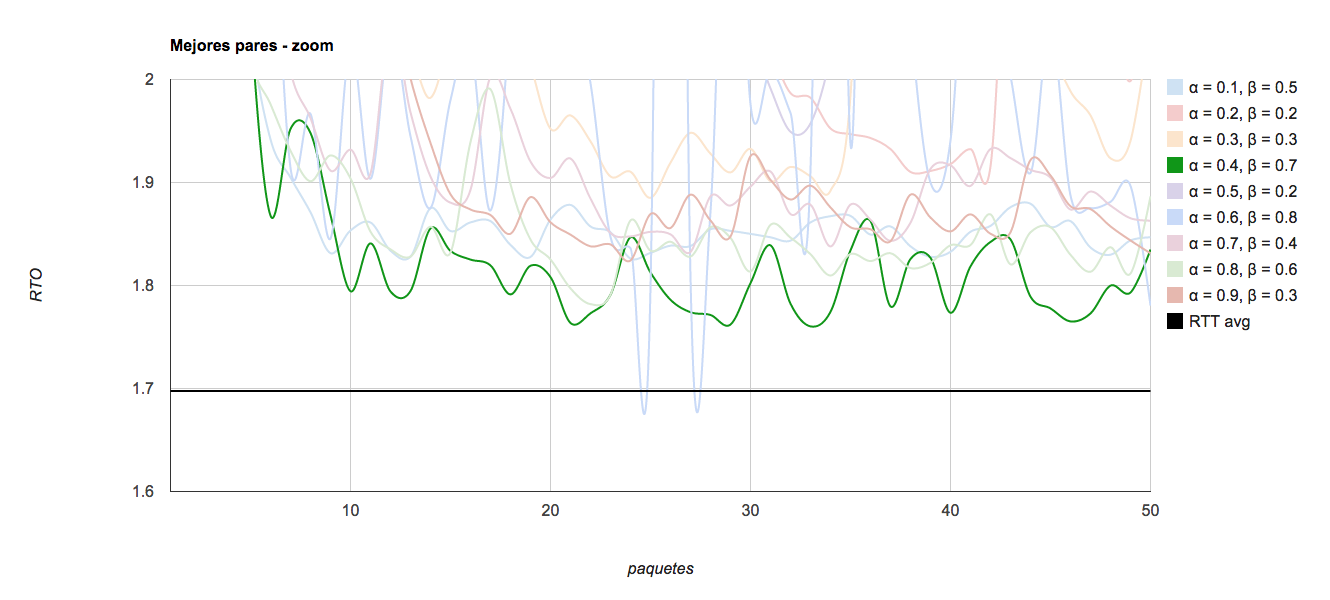
\includegraphics[scale=0.35]{graphics/best_pairs_zoom.png}
	\textit{Gráfico interactivo en:} http://goo.gl/RvuVpr
\end{center}

Para los próximos experimentos, utilizaremos estos que hemos determinado como mejores pares de $\alpha$ y $\beta$ para analizar como se comportan los mismos cuando se agrega la nueva variable de \textbf{probabilidad de dropeo} de un paquete.

\subsection{Experimento 2}

\begin{center}
	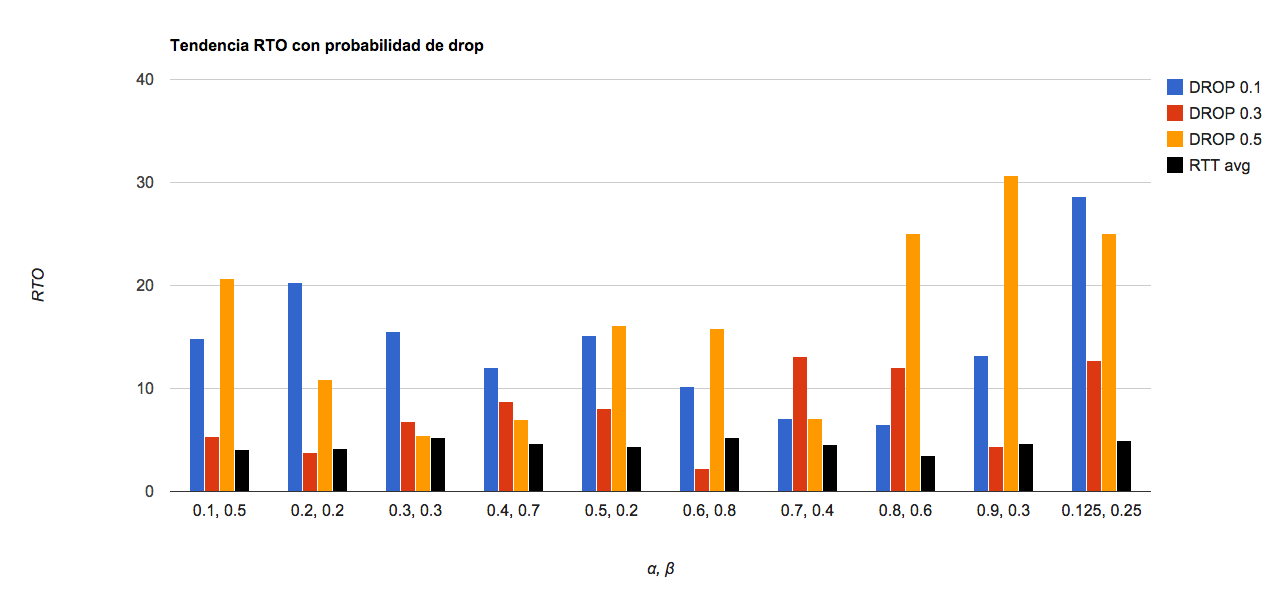
\includegraphics[scale=0.35]{graphics/tendencia_RTO_drop.png}
	\textit{Gráfico interactivo en:} http://goo.gl/6aM368
\end{center}

\begin{center}
	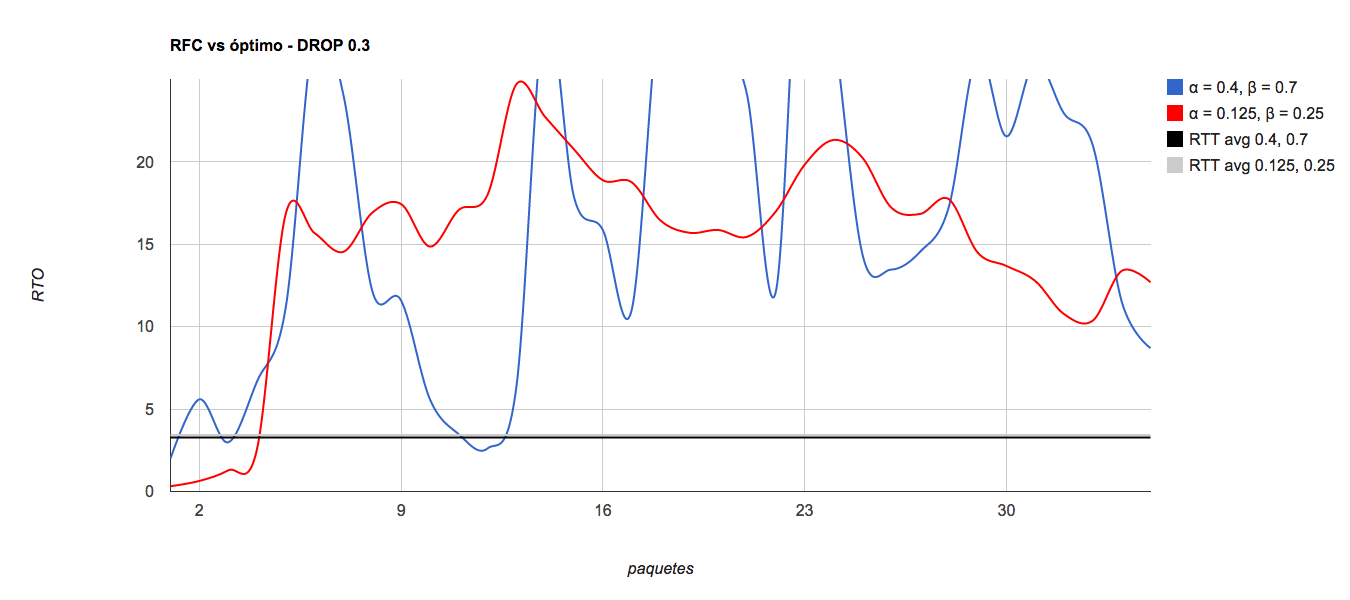
\includegraphics[scale=0.35]{graphics/rfc_vs_optimo.png}
	\textit{Gráfico interactivo en:} http://goo.gl/jaEjFw
\end{center}
